\chapter{绪论}
\section{研究背景与意义}
随着信息技术的发展, %wb
软件日渐成为人民生活、经济发展过程中不可缺失的基础设施, %sb
软件安全对
国家的经济、政治、国防以及个人隐私有着不可估量的重要影响。
%软件安全已不再是单点孤立的安全问题。
互联网技术将国家的文化、科技、艺术、宗教等意识形态领域的边界直接延展到人们的日常生活当中,传统的国土资源边界已被扩展至整个网络资\upcite{noauthor_autodafe_nodate}源空间,无论是对在政府、金融、通信、交通、贸易、物流、能源等国家核心基础设施的保障还是对涉及个人隐私的信息资料的保护无不依赖于软件的可靠性和安全性。然而,由于软件安全漏洞的广泛存在,给网络犯罪分子留下可乘之机,制造出的网络犯罪案件层出不穷,导致个人隐私曝光、商业机密泄露、重大经济损失或关键系统被恶意操纵。

%syf
由于软件漏洞的普遍性和高危害性,各国政府都十分重视软件漏洞的相关研
究。2003 年,美国政府发布的国家安全战略报告《The National Strategy to Secure
Cyber space》指出了网络安全防御面临的诸多问题,重点指出由软件安全漏洞问
题引发的严重后果,特别强调了网络和软件安全漏洞问题的重要性。2013 年,美
国国防高级研究计划局(DARPA)启动了一项预算达 5500 万美元的 Cyber Grand
Challenge(CGC)项目,旨在构造一个自动推理系统,自动发现软件中存在的漏
洞并修补它们。我国在 2006 年发布的《2006-2020 年国家信息化发展战略》第四
章“我国信息化发展的战略重点”中明确指出:“积极跟踪、研究和掌握国际信息
安全领域的先进理论、前沿技术和发展动态,抓紧开展对信息技术产品漏洞、后
门的发现研究,掌握核心安全技术,提高关键设备装备能力,促进我国信息安全
技术和产业的自主发展”。
%syf

%wb
%人们通常以软件漏洞造成的经济损失来强调软件
%漏洞的影响,但自“震网”病毒、“火焰”病毒之后,人们发现软件漏洞远不是经
%济损失可以衡量的,软件漏洞已成为网络空间博弈的关键资源。
%wb
%syf
尽管软件安全问题得到极大重视,相关软件开发企业和研究机构等都投入了
大量人力、物力去保证软件产品的安全性,
%syf
但因漏洞引起的严重的安全问题还时有发生。例如,2014年OpenSSL加密库被曝出的“心脏出血”(Heartbleed)漏洞影响了全球近1/3的主要网站;同年,与“心脏出血”同级别的破壳漏洞(ShellShock)被曝出,大约有5亿联网设备以及网络服务器受其影响;2015年glibc库的DNS客户端被曝出存在缓冲区溢出漏洞,全球数以万计的app、系统以及嵌入式设备收到影响。
%每年CVE都会曝出很多漏洞,
%说明当前的漏洞挖掘手段还不能满足实际的需求,仍然存在很大的提升空间,需要进一步深入研究。 %syf



%信息时代一大特点在于信息技术贯穿了人类的社会生活,支撑着经济、文化、科研、政府监管和工业生产等各方面的发展。软件作为信息系统中的核心基础设施,已广泛应用于航天、工控、汽车、电器、交通、医疗、能源、金融等领域,成为日常生活中不可或缺的一部分。

%软件故障缺陷是指会导致系统崩溃的软件错误,其形成原因主要包括内存泄漏、资源泄漏、空指针使用错误、数组越界、非法计算、使用未初始化变量、死循环结构和死锁等。软件安全漏洞会给系统留下安全隐患,导致系统被攻击。该类错误为他人攻击软件提供可能,一旦软件被攻击成功,可能造成系统被攻击者所完全控制,其危害更严重。安全漏洞成因主要包括未验证的输入、滥用API、安
%全功能部件、竞争条件、不合理异常处理、缓冲区溢出、代码质量和封装不当等。

%软件故障缺陷曾经引发多起灾难性事故,带来非常严重的损失。例如:1985年至1987年,由加拿大原子能有限公司制造的Therac-25放射治疗仪设备,由于系统和软件的安全性设计方面存在严重问题,共造成6起超剂量辐射事件,造成4人死亡,2人重伤;
%抄的
%1996年6月,在欧洲Ariane五型火箭的首次发射中,由于惯性参考系统软件的数据转换错误引起操作失误,致使火箭在发射40秒后爆炸,造成25亿美元的经济损失;2002年美国NIST估算,美国每年因软件失效所造成的年度经济损失近600亿美元,约占其GDP的0.6\%;2003年8月,美国电力检测与控制管理系统中的软件失效,造成美国东北部大面积停电,损失超过60亿美元;2004年9月,由于空管软件中的时钟管理缺陷,美国洛杉矶机场400余架飞机与机场指挥系统一度失去联系;2005年11月,日本东京证券交易所由于软件升级出现系统故障,导致股市停摆;仅2006年,中航信离港系统就发生了三次软件系统故障,造成近百个机场登机系统瘫痪;2006年4月,中国银联跨行交易系统出现故障,使整个交易系统瘫痪约 8 小时。
%抄的

随着各种开源社区的兴起,源代码组件在开源和商业软件中得到了广泛的应用,源代码软件漏洞的影响也越来越大。有研究表明\upcite{noauthor_78_nodate},超过半数的全球500强企业使用有漏洞的开源组件或者对开源库进行重新封装。另外一份来自Aspect Security的调查报告\upcite{williams_unfortunate_2012},审查了来自60000个企业、政府以及非盈利机构企业使用的网站和业务软件,发现超过半数的机构下载和使用了有漏洞的开源组件或者开源库,同时发现在调查之前绝大部分漏洞未得到修补。所以无论是商业软件还是程序员自行开发的小程序,开源代码已经变得越来越普遍,而且开源也已经成为了一种趋势。商业软件项目的免费版本数量已经超过了50\%甚至更多,而开源软件产品所占比重从2011年的3\%增长到了现在的33\%。平均每一款商业软件都会使用超过100个开源组件,而且三分之二的商业应用代码存在已知安全漏洞。Black Duck软件公司的研究人员根据他们对开源项目所收集到的统计数据预测到,基于开源软件漏洞的网络攻击活动数量在2017年将增长20\%。

随着软件功能的日益增多和规模的日益庞大,软件存在故障缺陷和安全漏洞不可避免。
源代码软件的漏洞挖掘技术能够针对性的对开源软件/组件进行挖掘,其研究一方面能够提升软件的安全性,对我国自主研发软件质量的提高具有重大意义;另一方面,随着开源软件/组件被国外军、政、企部门广泛的使用,对我国的漏洞资源储备以及网络空间博弈也具有重大战略意义。
%从而给信息系统的可靠性和安全性带来严重的威胁。
%随着国内外各种开源社区的兴起,

%源代码漏洞检测是软件发布之前最后的检测环节,对于软件安全具有重大意义。
%因为编程人员能力的参差不齐、程序开发过程中的疏忽以及应用程序的复杂性,导致软件中不可避免的出现编程错误和安全缺陷。
%相对于二进制程序,在获取更多信息的基础上,源代码软件的漏洞挖掘技术能够有针对性的对开源软件/组件进行挖掘,从而更高效的挖掘漏洞。
%虽然源代码软件漏洞挖掘已经发展了多年,但任然存在一些问题有待解决,例如无法进行多种类漏洞可疑区域标定、符号执行执行效率低以及模糊测试

%源代码软件的漏洞挖掘技术能够有针对性的对开源软件/组件进行挖掘,
%掌握开源软件的漏洞挖掘技术对我国、我军的信息安全具有重大战略意义。另外一方面,因为编程人员的编程能力参差不齐、编程过程中产生疏忽以及应用程序的复杂性,导致软件中不可避免的出现编程错误和安全缺陷。源代码漏洞检测是软件发布之前最后的检测环节,对于我国自主研发软件的安全具有重大意义。

\section{源代码软件漏洞挖掘研究现状}
%wb
%从不同的关注点出发,软件漏洞的内涵通常有所不同,论文理解的漏洞是指有可能导致软件或硬件出现异常的逻辑设计和实现上的缺陷、人为设计和实现的隐蔽功能以及因使用管理不当形成的安全隐患。

%软件漏洞挖掘方法按照测试时是否需要运行程序分为静态挖掘方法和动态挖掘方法。
\subsection{软件漏洞挖掘方法分类}
近年来,漏洞挖掘研究在理论方法层面不断更新,高效的挖掘工具层出不穷,
软件漏洞挖掘技术的划分方式也存在不同的维度。 %mqk
这些挖掘方法按照是否使用运行时信息有静态、动态之分;按照自动化程度不同有手工、自动之分;按照挖掘对象不同有面向源码和面向二进制之分。图\ref{根据挖掘方式分类}中可以看到:人工审计、崩溃分析、程序调试、逆向工程是典型的手工分析方法;补丁对比、语法/语义分析、模型检测、抽象解释是典型的自动化静态分析方法;错误注入、模糊测试、二进制插桩是典型的自动化动态分析方法;污点分析和符号执行也是自动化分析方法,在动态分析和静态分析中都有应用。图\ref{根据挖掘软件类型分类}中可以看到:语法/语义分析、模型检测主要用于面向源码分析;程序调试、崩溃分析、逆向工程、二进制插桩则主要用于面向二进制分析;人工审计、补丁对比、抽象解释、污点分析、符号执行、模糊测试、错误注入则在源码和二进制分析中都有应用。论文重点关注面向源代码的动态和静态自动化分析方法。

\begin{figure}[htb]
\begin{center}
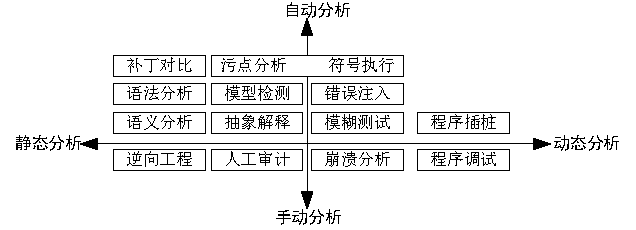
\includegraphics[scale=0.3]{chap01/根据挖掘方式分类}
\end{center}
\caption{根据挖掘方式分类}
\label{根据挖掘方式分类}
\end{figure}


\begin{figure}[htb]
\begin{center}
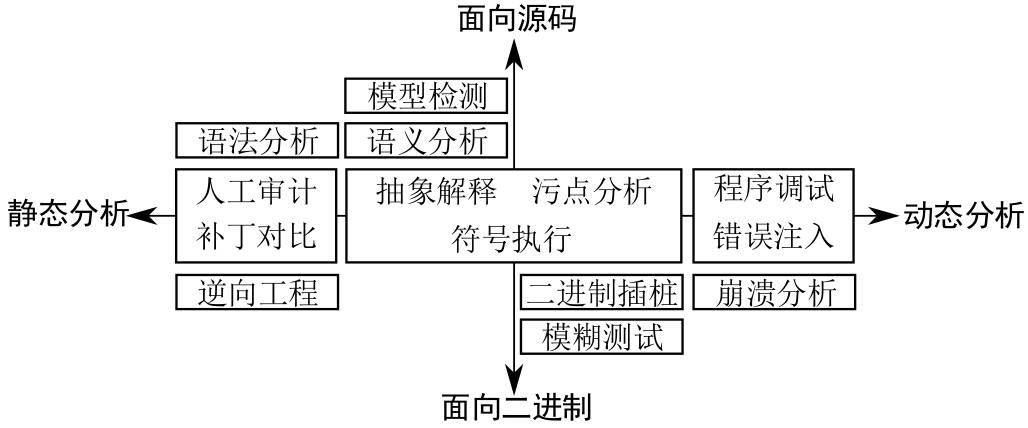
\includegraphics[scale=0.3]{chap01/根据挖掘软件类型分类}
\end{center}
\caption{根据挖掘软件类型分类}
\label{根据挖掘软件类型分类}
\end{figure}
%wb
\subsection{源代码软件静态挖掘技术}

静态挖掘技术是在不运行程序的情况下,自动的发现和报告潜在安全漏洞的技术的统称。静态分析能够全局的分析程序,不需要遍历每一个程序执行状态,从而扩大程序分析的规模。总体上,静态分析具有以下优点。(1)能够在软件生命周期的早期发现漏洞。静态分析可以在函数单元上进行单元测试,这使得错误可以在集成到大的代码模块之前被发现。进行单元测试之后,可以将精力集中在函数/单元之间的交互漏洞检测上,实现对源代码的分层检测。(2)能够检测大规模的软件。相对于人工审计,静态分析虽然压制了其报告解析能力,但是提高了检测特定漏洞的能力。相对于动态测试,不需要动态的遍历程序的每一个状态或者仅仅在源程序、中间表示上进行分析,能大大减少分析所需要的时间。同时静态分析也有以下不足。(1)在没有源代码的情况下,例如第三方库、操作系统等,静态分析需要猜测这些缺失的程序行为。(2)不能处理未域定义的程序错误行为。(3)不能检测运行时的漏洞、设计漏洞,系统管理以及由于用户的原因产生的漏洞。

%\begin{enumerate}[(1)]
%\item 能够在软件生命周期的早期发现漏洞。静态分析可以在函数单元上进行单元测试,这使得错误可以在集成到大的代码模块之前被发现。进行单元测试之后,可以将精力集中在函数/单元之间的交互漏洞检测上,实现对源代码的分层检测。
%\item 能够检测大规模的软件。相对于人工审计,静态分析虽然压制了其报告解析能力,但是提高了检测特定漏洞的能力。相对于动态测试,不需要动态的遍历程序的每一个状态或者仅仅在源程序、中间表示上进行分析,能大大减少分析所需要的时间。
%\end{enumerate}
%
%同时静态分析也有以下不足。
%
%\begin{enumerate}[(1)]
%\item 在没有源代码的情况下,例如第三方库、操作系统等,静态分析需要猜测这些缺失的程序行为。
%\item 不能处理未域定义的程序错误行为。
%\item 不能检测运行时的漏洞、设计漏洞,系统管理以及由于用户的原因产生的漏洞。
%\end{enumerate}

%大师兄
程序静态分析技术经过几十年的发展,形成了丰富的理论方法和技术手段,以程序静态分析为基础的静态漏洞挖掘方法的研究也极为深入。在词/语法分析、定理证明、抽象解释、符号执行、模型检验和机器学习等理论的支持下,静态漏洞挖掘取得了显著进展。
%大师兄

\subsubsection{词/语法分析技术}

词法分析通过对以往漏洞的分析,例如,人们发现缓冲区溢出常与某些语句或者语句组合有关(例如 strcpy, strcat),于是开发了一些通过词法分析发现缓冲区溢出漏洞的检测工具,例如 RATS\upcite{wnoauthor_cern_nodate}、 ITS4\upcite{noauthor_its4_nodate} 和Flawfinder\upcite{flawfinder_nodate} 等。此类工具对程序的语句进行遍历,并与预先建立的漏洞模式进行匹配,最后根据匹配结果报告可能的缓冲区溢出漏洞。由于这种方法不理解程序语义,所以容易产生漏报或误报。此技术一般只作为手工分析的起点。

\subsubsection{定理证明方法}

定理证明的基本思想是将源程序的语义和安全规范转换为逻辑公式,再将这些逻辑公式输入到一个定理证明器进行验证,从而将软件错误的发现过程转换为逻辑公式的证明过程。这种方法的优点是严格,能够保证通过验证的程序不存在漏洞,但它通常要求用户( 用形式逻辑语法) 提供循环不变式、过程调用的前置条件和后置条件等信息,以帮助定理证明器完成推导,因而难以实现自动化。Compaq 公司的 ESC\upcite{leino_esc/java_2000}、以色列 Tel-Aviv 大学的 CSSV\upcite{dor_cssv:_2003} 都采用定理证明方法检测程序中的缓冲区溢出漏洞。

\subsubsection{抽象解释技术}

抽象解释把程序的执行过程看成抽象状态的迁移过程,并通过抽象状态的分析确定程序的性质。为了保证分析结果的正确性,抽象解释要求初始抽象状态是初始实际状态的安全近似,且每次状态迁移都能保持正确关系。正确的抽象解释能够发现程序中的漏洞,但存在较多的误报,所以在实际使用时常常要求用户根据被测试程序的特性,选择合适的抽象域、加宽操作和解释函数等,以降低误报率。例如, Patrick Cousot 领导的项目 ASTREE\upcite{cousot_astree_2007} 采用基于抽象解释理论的程序静态分析器。ASTREE 可以检测数组越界访问、除零异常、浮点运算溢出和整数运算溢出等问题。ASTREE曾用于检验法国空中客车公司的空中巴士A340和A380系列飞机飞行控制软件,受到工业界的认可。除了ASTREE,FLUCTUAT\upcite{delmas_towards_2009} 、Coverity\upcite{almossawi_analysis_2006} 等都是采用抽象解释理论进行静态
漏洞检测的典型工具。抽象表达提供了对变量边界值的估计,但无法有效追踪变量之间的约束关系,在路径可行性判定上依然存在不足。

%\subsubsection{约束分析}
%
%约束分析是一种通过建立和求解程序的约束条件,发现程序性质的方法。基于约束分析的静态方法常将检测过程分为约束产生和约束检查两个独立步骤,前者利一组约束产生规则建立程序的约束条件,后者对建立的约束条件进行求解,进而检验程序的性质。约束分析可以处理无穷系统,而且自动化程度较高。美国加州大学Berkeley分院的 Wagner设计了一个基于约束分析的缓冲区溢出漏洞检测器BOON\upcite{noauthor_boon_nodate}。

\subsubsection{静态符号执行技术}

静态符号执行是King等人1976年在文献\upcite{king_symbolic_1976}一文中首先提出。符号执行的基本思想是,用抽象的符号表示程序中变量的值,根据程序的语义,遍历代码执行空间,来模拟程序的执行。符号执行的主要优势在于能够发现变量之间运算关系,便于理解程序的内在逻辑;在漏洞挖掘时,有利于在复杂的数据依赖关系中发现数据之间本质的约束关系,而且符号执行精确记录了路径的约束条件,可以进一步用于判断路径可行性和路径约束的完备性。

符号执行技术通过将程序的输入由具体值替换为符号变元,将程序中每条指令本身的具体计算语义映射为相应的符号计算语义,在程序控制流指导下,关注路径的分支谓词,为路径状态树中的每个叶子节点对应的程序路径推导出相应的能够到达该位置的敏感输入满足的最弱前条件。符号执行的核心,在于以等价类的形式对程序的执行路径进行标注,进而高效率地实现路径覆盖。

符号执行可以分析代码的所有语义信息,也可以只分析部分语义信息。符号执行分为过程内分析和过程间分析(又称全局分析)。过程内分析是指只对单个函数的代码进行分析,全局分析指对整个软件代码进行上下文敏感的分析。所谓上下文敏感分析是指在当前函数入口点要考虑当前的函数问调用信息和环境信息等。程序的全局分析是在过程内分析的基础上进行的,但过程内分析中包含了函数调用时就也引入了过程问分析,因此两者之间是相对独立又相互依赖的关系。

符号执行常常在对路径敏感的程序分析中使用。符号执行可以看作是程序测试与程序验证的折中方法,其优点在于它可以精确地静态模拟程序的执行。由于它跟踪了变量的所有可能取值,因此能够发现程序中细微的逻辑错误。但是在处理大程序时,程序执行的可能的路径数目随着程序尺寸的增大而呈指数级增长。在这种情况下需要对路径进行选择,选取定数量的路径进行分析。

早期静态符号执行典型系统包括Prefix\upcite{bush_static_2000}和ESP\upcite{das_esp:_2002}。W.Bush等人在1998年提出了Prefix,并在美国申请了若干专利。微软公司于1999年收购了Prefix,在Prefix基础上实现了Prefast。Prefix/Prefast已经成为微软内部标准源代码静态检验工具之一。ESP借鉴了MC由用户制定检查规则的思想,基于符号执行技术识别和保留路径上安全属性状态相关的约束条件,能够有效排除很多不可行路径。

\subsubsection{模型检测技术}

模型检验是一种针对有限状态并发系统的自动分析与验证技术,其基本思想是状态搜索。对状态空间的穷尽搜索有赖于对系统建立的有穷状态模型,以保证搜索过程的终止。模型检测的优点是能够做到完全自动化,在搜索终止时,如果性质没有满足,能够给出反例,这有利于用户对系统进行改进; 缺点是建模比较困难,且面临状态空间爆炸的问题。一般情况下,模型检查只适合用于对临时属性(如内存是否被释放、指针是否为空等)的检测。

模型检验技术最早应用于时序电路和通信协议设计的自动化检验,其基本思想是用状态迁移系统描述程序的行为,用时序逻辑、计算树逻辑或π演算公式表示系统的性质,从而将系统属性的检验问题转换为搜索不满足逻辑公式的状态系统的问题。模型检验需要遍历系统的整个状态空间,所以只能分析有限状态系统。例如,Berkeley大学的MOPS\upcite{chen_mops:_2002}、微软研究所的SLAM以及Bell实验室的UNO\upcite{holzmann_static_2002}都是基于模型检验的检测工具,它们能够发现程序中的一些字符串库函数的滥用。MOPS系统能够做到检测结果无漏报(完备性),但是MOPS是数据流不敏感的分析,无法跟踪数据依赖关系,导致MOPS误报率很高。SLAM\upcite{noauthor_slam_nodate}是一种基于谓词抽象技术的软件模型检验器,主要用于检测Windows操作系统驱动程序是否满足用户定义的属性约束。SLAM的核心技术是谓词抽象,将每个变量都抽象为只有0/1两种取值。这种过近似(Over Approximations)抽象方法导致SLAM误报较为严重。由于模型检验技术面临着状态空间爆炸的问题,在大型复杂软件的漏洞挖掘工作中仍处于探索阶段。

有些模型检验工具,例如Spin\upcite{noauthor_spin_nodate}与CBMC\upcite{noauthor_cbmc_nodate},能够直接应用于源代码,准确地捕捉程序的真实行为,精确度比较高。但是,它们要么可扩展性不好,不能应用于大规模的程序(如Spin);要么只能检查大型程序的部分状态,用作一种查错工具,不能覆盖所有的状态,不能保证找到所有的错误。另外一些模型检验工具基于谓词抽象的思想自动化抽取系统的有穷状态模型,如BLAST\upcite{beyer_software_2007}和SATABS等,它们的基本思路都是谓词抽象与CEGAR(Counter Example Guided Abstract Refinement,反例制导抽象精化)\upcite{andraus_cegar-based_2007},这也是目前主流的软件模型检验实现思路,但谓词发现以及模型精化仍是此类技术中的难点问题。


\subsubsection{基于机器学习的软件漏洞静态挖掘技术}
%随着机器学习算法的成熟,机器学习的很多方法也应用到了漏洞挖掘和软件测试之上。例如智能优化算法在模糊测试技术上的应用,AFL-go\upcite{bohme_directed_2017}利用模拟退火算法随着时间的推移分配种子变异的能量;AFL\upcite{noauthor_american_nodate}利用遗传算法框架变异种子以扩大测试的代码覆盖率;另外还有将遗传算法应用到回归测试\upcite{doungsa-ard_automatic_2007}、基于模型的模糊测试技术\upcite{sharma_applying_2014,sabharwal_prioritization_2010,you_genetic_2012,patton_genetic_2003}以及web测试\upcite{peng_new_2011}当中。

随着机器学习算法的成熟,一些研究者将机器学习的有监督、无监督算法以及神经网络算法和程序分析相结合用于挖掘软件漏洞。Padmanabhuni\upcite{padmanabhuni_predicting_2014,padmanabhuni_auditing_2016}利用有监督机器学习算法建立分类器用以检测缓冲区溢出漏洞。Neuhaus\upcite{neuhaus_predicting_2007}根据Mozilla的漏洞历史,从中提取向量,并利用机器学习算法预测哪些组件有可能出现漏洞。Zimmermann\upcite{zimmermann_searching_2010}以代码复杂度、代码混淆度等为特征预测Windows Vista中可能出现漏洞的组件。Perl\upcite{perl_vccfinder:_2015}利用github提交代码的语言类型、贡献者的fork数量等特征预测哪些提交可能出现漏洞。Grieco\upcite{grieco_toward_2016}以C语言程序中的函数调用轨迹为特征预测大规模程序中的漏洞。Yamaguchi\upcite{yamaguchi_chucky:_2013,yamaguchi_automatic_2015}利用异常检测检测源代码中缺少边界检测的情况以及使用聚类算法检测Taint-Style类型的漏洞。Rajpal\upcite{rajpal_not_2017}提出了一种基于时间递归神经网络的提高模糊测试代码覆盖率的方法。


\subsection{源代码软件动态挖掘技术}

动态测试是对程序运行时特性的测试分析,有别于静态分析检查源程序的手段,动态分析通过检查运行时的程序来获取程序特性。静态分析的结果通常对于每次程序的执行都成立,而动态分析的结果可能只对某一次或某几次运行成立。动态分析正在被广泛应用于包括系统安全分析在内的多个领域,软件工程国际会议(International Conference on Software Engineering/ICSE) 专门设立了动态分析研讨会( Workshop on Dynamic Analysis/WODA),会议的主题包括动态分析的各种研究和应用。

\subsubsection{运行时监测技术}

运行时监测(Runtime monitoring)是根据插桩的安全规范代码和检测代码在程序运行时检测是否违反安全规范。如斯坦福的Michael Martin等人的PQL(program query language)\upcite{martin_finding_2005},首先使用上下文敏感、流不敏感、基于包含的指针别名分析,找出所有可能的匹配点,然后对这些匹配点进行插桩后在运行时监测。另外像VS.Net 中使用的放在调用栈中的canary,canary值存放在用户数据和返回地址之间,一旦发现canary值被改变,则表明发生了缓冲区溢出。运行时监测首先要利用各种静态分析技术(如指针分析、别名分析、类型推断等),结合给出的安全规范,找出程序中所有可能违反安全规范的地方;然后利用代码插桩技术(包括静态插桩和动态插桩)对可能出现安全漏洞的地方插桩检测代码,同时插桩安全规范;最后利用动态检测算法在运行时检测程序是否违反安全规范。

\subsubsection{动态符号执行技术}

%\textbf{参考directed Greybox Fuzzing的introduction中关于符号执行的介绍}

基于动态符号执行的漏洞挖掘,一般将关注的程序漏洞以符号断言的形式进行描述。对每条路径的符号分析过程中,在敏感的程序点处对漏洞断言的可满足性进行判定。如确定断言为可满足,即断定当前分析路径中存在该类型漏洞。近年来,该型技术得到了较为广泛的应用。

2005年,Godefroid等学者提出的DART\upcite{godefroid_dart:_2005}系统是最早的动态测试用例生成系统。DART首先生成一个随机值作为外部变量的初始化输入,且对每个外部函数都返回一个随机值,由于随机值不能确保对程序中的每条分支都能覆盖到,因此随机测试的覆盖率通常很低。然而,DART对输入的随机值进行符号化处理,即在随机化之后,这些变量被标记为符号变量。在遇到新分支时,一条路径约束通过不断收集执行过程中的约束来生成,而下一条路径则是通过对另一分支的约束取反来生成。如果一条路径不可求解,这个约束将用具体值代入,进行化简。DART的缺点时不能处理指针语义,无法分析C语言中常见的指针操作。

CUTE\upcite{sen_cute_2006}被定义为一个混合符号执行工具,即联合了符号执行与具体执行。与DART系统类似,CUTE允许用户通过指定代码来决定哪些输入可以被符号化,这使得任意外部用户输入都可以被替代。CUTE的路径遍历是通过插桩来实现的。与DRAT相比,CUTE最大的改进是能够处理指针操作和数据结构。

斯坦福大学的Engle等学者提出的EXE\upcite{cadar_exe:_2008}系统,用于组件测试,在动态收集路径可达约束信息方面和约束路径精确求解方面的贡献较为突出。EXE系统是一个源到源的编译器。该编译器将目标应用源码中的每一个赋值和运算前都插入对EXE系统符号化执行组件的函数调用,并在程序的分支语句前插入一段调用求解器代码,对当前分支条件进行求解并产生测试用例。这样,当被EXE编译后的程序真正执行时,真实的程序执行和符号化执行交替进行,并且符号化执行从程序的具体执行中获取所需运行时信息,以收集路径可达约束。此外,EXE系统实现了一个SMT求解器 STP,该求解器包含了BV理论、ARRAY理论和整数理论。由于路径可达约束的收集和约束求解都较为精确,EXE系统生成的测试用例软件缺陷的发掘效率较高。

KLEE\upcite{cadar_klee:_2008}系统是基于EXE系统的升级,该系统将EXE系统的源到源编译器变为LLVM编译器\upcite{noauthor_llvm_nodate}。KLEE系统纯符号化执行LLVM编译出的低级指令。这些改进使得KLEE系统可以更为普适地应用于各类LLVM支持的语言程序。KLEE同样需要完整源码支持。并且由于KLEE系统采用完全符号化解释执行每一条LLVM指令,测试性能低。

SAGE\upcite{godefroid_sage:_2012}系统是微软研究院研发的动态测试用例生成系统。与之前的系统不同,SAGE系统直接对二进制程序进行动态追踪并生成测试用例。该系统采用动态二进制指令追踪工具Nirvana,监控程序执行,追踪指令执行获得程序的执行流日志。然后再离线地对日志文件进行符号化分析执行,构建路径可达约束,以便为输入可控分支生成测试用例。与EXE系统不同,SAGE系统为了能够对大规模程序进行分析,采取了一系列的简化措施:(1)SAGE系统为了简化约束收集和求解的复杂性,忽略对非线性约束的收集与求解。(2)SAGE 系统不对程序中的指针进行分析。相对于EXE系统,以上简化措施一定程度上加快了SAGE系统对大型目标软件的测试用例生成速度,然而这却以损失测试用例对路径覆盖指导的精度为代价。SAGE系统生成的测试用例中有接近60\%的测试用例无法准确指导程序覆盖目标路径。此外,SAGE系统对日志中的所有指令流都采用完全符号化解释执行,导致符号化执行时间占全系统工作时间的25\%。这就抵消了部分由前面所述简化操作带来的性能提升。

伯克利大学的SmartFuzz\upcite{molnar_dynamic_2009}系统与SAGE系统类似,采用了基于Linux下的二进制指令追踪工具Valgrind追踪程序执行和在线约束收集方式。SmartFuzz系统仅支持整数溢出缺陷的发掘。

李根设计和实现了Hunter\upcite{hunter__2010}系统,提出了基于路径完备可达理论以及污点可控指针分析的算法,能有效覆盖基于攻击面污点输入可达的测试路径,由于采用了基于虚拟机平台的符号化执行及线程监控技术,具有良好的跨平台兼容性。

在符号执行的实际应用中,还面临这许多问题,比如符号执行的精度
问题\upcite{godefroid_higher-order_2011},复杂的输入格式问题\upcite{majumdar_directed_2007,godefroid_grammar-based_2008},路径爆炸问题\upcite{boonstoppel_rwset:_2008,godefroid_compositional_2010},符号指针问题\upcite{trtik_symbolic_2014}等。其中路径爆炸问题是一个符号执行研究的一个重要分支。其主要形成原因在于,每一个分支条件语句都可能导致当前路径再分支出一条新的路径进行分析计算,而这是以指数的形式增长的。尤其体现在程序中存在跳转谓词与输入变元相关的循环结构时。

当前的解决办法包括:为循环引入“执行计数变量”,通过进行“执行计数变量”与输入的关联和程序中的变量与“执行计数变量”的关联,实现将程序中“循环次数相关”的变量的值完全通过输入相关属性表达的抽象计算。作为一种
摘要计算技术,约减了循环处理中的分析计算量;在对大量实际应用程序分析的基础上,仅仅为输入的“长度”和“部分输入前缀字符”引入符号变元,进行符号计算。该方法理论上并不是完备的,但实际应用中能覆盖较多的缓冲区溢出情形;有些相关研究提出综合使用程序切片、抽象解释、循环不变量计算和循环单值识别等技术对循环执行次数的上界进行估算:利用程序切片获取与循环结束判断条件相关的变量和语句,进而在此基础上进行抽象解释,对相关变量的取值范围近似获取。在经过循环不变量分析和循环单值识别后,进一步剔出变量值域,最终获取循环次数的估计值。

Godefroid等在文献中通过为包含归约变量的输入相关的循环计算循环摘要\upcite{godefroid_automatic_2011},避免了对每条循环相关分支的分析。但仅仅适用于循环中变量与归约变量存在线性关系的情况下;瑞士的开源项目S2E\upcite{chipounov_s2e:_2011}提出了选择式符号执行的思路:仅仅对关注的程序部分(某一特定代码模块或访问某一特定数据的代码部分)进行符号执行,在关注的程序部分和不关注的程序部分之间,维护确保分析状态一致性的转换机制。

%\subsubsection{导向符号执行技术}

导向符号执行是符号执行中利用程序分析以及约束求解技术有效的搜索可能目标路径空间的一个方向\upcite{ma_directed_2011}。Haller\upcite{haller_dowsing_2013}提出了一种导向危险库函数以及危险操作的区域的符号执行方法。另外一些研究者将导向符号执行应用到程序补丁验证\upcite{bohme_partition-based_2013,marinescu_katch:_2013,miller_empirical_1990}、增加符号执行代码覆盖率\upcite{xu_directed_2010}、减少静态分析误报\upcite{christakis_guiding_2016}以及崩溃重现之上\upcite{jin_bugredux:_2012, ros_sler_reconstructing_2013}。但是导向符号执行是重量级的,需要大量的程序分析以及约束求解。

%\subsubsection{约束求解技术技术}
%
%使用动态符号执行进行测试数据生成的基础在于底层的约束求解技术一一预期的程序路径约束最终需要表达为约束求解器所识别的语言,并由其判断可满足性以及给出对应的数据样本。
%
%lp\_solve\upcite{buttrey_calling_2005}是一个开源的线性规划求解器,其可以求解纯线性、整型、半连续及Special Ordered Sets\upcite{beale_global_1976}模型。我们将路径约束的求解问题转化为了在路径约束变量上的线性规划问题。虽然lp\_solve的求解能力不足以覆盖一般程序中出现的所有运算操作,如乘法、除法、位运算,但是已经足够覆盖足够的范围,即并行化现有方法。
%
%另一方面,如果需要表达能力更强的约束求解器,则可以选择SMT(Satisfiability Modulo Theories)\upcite{ranise_satisfiability_2006}求解器。SMT问题是布尔可满足性问题的扩展,前者将后者公式中的布尔变量替换为了由不同底层理论(如整型、实数、位向量甚至是不同的复杂数据结构)所支撑的谓词。因而,相比其他可用于约束求解的技术而言,SMT求解器有着更加强大的表达能力。当前的SMT求解器可直接支持包含如数组、结构体、枚举量之类的真实程序中经常出现的数据结构的模型,而避免了由包含这些结构的程序路径约束向表达能力较弱的求解器语言转换时可能导致的语义丢失。
%
%STP(Simple Theory Prover,简单理论证明器)\upcite{noauthor_simple_nodate}是用于求解定长比特向量和一维数组的逻辑公式可满足性的决策程序。简单的说STP就是一种用于求解特定逻辑方程组的工具。STP有其自身的语言规范,包括提供的接口函数和语法规则。接口函数包括比特向量的拼接和抽取、移位、符号扩展、有符号和无符号的算术操作(加减乘除取模等)和逻辑位操作等。还提供了比特向量间的有/无符号比较谓词(大于等于小于)。
%
%只要符号执行提取的路径条件符合 STP 的语法规范,就可以利用 STP 进行求解,从而判断一条具体的路径是否成立,如成立,则可得到对应该路径的测试用例。

\subsubsection{模糊测试技术}

Miller等\upcite{miller_empirical_1990}在1991年首次提出了模糊测试的概念,目的是检测UNIX命令行工具程序的可靠性。因为事先不知道程序、输入的结构信息,最先的模糊测试被称为黑盒模糊测试。模糊测试通过不同的方式(例如比特反转、边界值替换、输入块删除和复制)变异程序输入,从而产生大量的畸形输入;然后将畸形输入反馈给程序执行,观察程序是否异常。这个简单且有效的方法奠定了模糊测试的基础。下面从三个方面概述模糊测试技术。

(1)基于模型的黑盒模糊测试技术

传统的黑盒测试\upcite{noauthor_zzuf_nodate}没有考虑输入的结构信息,以至于变异的绝大部分输入因为不符合正确的格式标准而只能检测程序的一小部分路径。这种情况导致了传统的黑盒模糊测试不能挖掘程序的深层次信息。为了解决这个问题,研究者提出了基于模型的黑盒模糊测试框架例如Peach\upcite{noauthor_peach_nodate}和Spike\upcite{noauthor_immunity_nodate}。本质上,当输入是有格式的文件数据或者协议数据时,测试用例变异需要保证程序输入能够满足格式规范,从而通过程序的格式检测。这种方法增加了生成的测试输入的有效性,从而能够测试更深更关键的程序状态。但是,有的文件或报文格式并未公开,如何获得准确的输入格式或者绕过对输入格
式的校验成为研究的重点问题\upcite{li_automatic_2011,kim_efficient_2011,gorbunov_autofuzz:_2010,lin_automatic_2010,wang_taintscope:_2010}。另外还有一些研究者将遗传算法应用到基于模型的黑盒测试技术当中\upcite{sharma_applying_2014,sabharwal_prioritization_2010,you_genetic_2012,patton_genetic_2003}。

%随着机器学习算法的成熟,机器学习的很多方法也应用到了漏洞挖掘和软件测试之上。例如智能优化算法在模糊测试技术上的应用,AFL-go\upcite{bohme_directed_2017}利用模拟退火算法随着时间的推移分配种子变异的能量;AFL\upcite{noauthor_american_nodate}利用遗传算法框架变异种子以扩大测试的代码覆盖率;另外还有将遗传算法应用到回归测试\upcite{doungsa-ard_automatic_2007}、基于模型的模糊测试技术\upcite{sharma_applying_2014,sabharwal_prioritization_2010,you_genetic_2012,patton_genetic_2003}以及web测试\upcite{peng_new_2011}当中。

(2)覆盖率导向的模糊测试技术

覆盖率导向的模糊测试是通过一系列方法增加种子语料库代码覆盖率的技术。其出发点是基于这样一个判断“如果要检测某个程序元素$e$中的漏洞,种子语料库中就必须要包含一个种子在程序执行时能够到达$e$”,这里$e$可以是一个语句、一个基本块或者其他的区域。在执行一个测试用例时,覆盖率导向的模糊测试工具\upcite{bohme_coverage-based_2016,noauthor_american_nodate,rawat_vuzzer:_2017,sparks_automated_2007,noauthor_libfuzzer_nodate}使用轻量级的代码插桩在运行时收集代码覆盖信息。AFLFast\upcite{bohme_coverage-based_2016}设计了一种路径概率计算方式,变异概率较低的路径对应的测试用例能触发更多的路径,从而增加代码覆盖率。同时,设计一种测试用例变异能量分配方式,驱动模糊测试多变异遍历概率低的路径。Vuzzer\upcite{rawat_vuzzer:_2017}为每一个基本块设置了一个权重,并且计算每条路径的权重,在模糊测试时着重测试更可能触发漏洞的路径。Sparks\upcite{sparks_automated_2007}使用了遗传算法的思想变异定长的种子语料库并根据输入数据格式以遍历更深的路径。

(3)目标区域导向的模糊测试技术

目标区域导向的模糊测试是指在指定目标区域的情况下,通过设定一系列标准,驱动模糊测试执行到目标区域的技术。Marcel Böhme在AFL的基础上开发了AFL-go工具\upcite{bohme_directed_2017}。该工具定义了每个测试用例和目标区域的距离,并设计一种基于模拟退火的能量分配策略,使得随着时间的增加到目标区域距离较小的测试用例变异次数增加,而到目标区域距离较大的测试用例变异次数减少,以此增加测试用例经过目标区域的概率。虽然AFL-go在一定程度上实现了导向性,但是其变异的方式依然是无序的。基于此分析,论文第五章提出了一种细粒度变异的导向模糊测试方法,根据关键字段权重变异测试用例以达到快速导向并发现更多漏洞的目的。

还有另外的研究者提出了基于污点分析的导向模糊测试技术\upcite{henderson_decaf:_2017, newsome_dynamic_2005}。该技术利用污点分析方法判断哪些字段对导向目标区域具有关键作用,变异这些字段产生的测试用例能够以更大的可能性遍历到目标区域。通过这种方式能够极大的减少需要遍历的程序状态空间。

%\upcite{meng_assisting_2017}

\section{源代码软件漏洞挖掘的关键问题}

%静态分析和动态分析是源代码软件漏洞挖掘的两个主要方向。
通过对比分析现有的源代码软件漏洞挖掘方法及工具,可发现源代码软件漏洞挖掘存在以下发展趋势\upcite{zhangliyong_2011}。%抄源代码安全性分析
\begin{enumerate}[(1)]
\item 从内置安全规则到可扩展安全规则。现在的源代码安全分析工具都会提供多种配置机制和接口,供分析人员根据实际需要编写程序实现自定义的安全分析\upcite{noauthor_code_nodate,ashcraft_using_2002}。
\item 从依靠抽象语法树的词法匹配的方式到到多中间表示混合匹配的方式。抽象语法树只能识别出程序中的敏感操作,且会产生大量的误报,将其他的中间表示形式,如控制流图和数据流图综合考虑能大大减少误报。
%\item 从单类型源代码漏洞分析到多类型漏洞分析。
\item 从单纯的程序员指导程序分析到以程序员为辅助的自动程序分析。程序员在安全分析中的参与比重越来越小。现在许多模型检测、抽象解释工具的使用,只需要程序员在可能发生漏洞的区域添加注释就可以完成。而另外一些分析工具\upcite{gregor_stllint:_2006,noauthor_splint_nodate},因为使用了更为复杂的语义提取方式,程序员的参与度进一步减少。
\item 使用形式化方法辅助软件测试。软件测试方法本质上是遍历程序状态空间,容易引起状态空间爆炸。形式化方法通过提供语义等价的程序转换,能够减少状态空间。将二者结合,能够发现软件测试检测不了的漏洞。
\item 使用源代码的直接或者间接信息辅助软件测试。越来越多的从源代码中获取的信息用于帮助符号执行、模糊测试等软件测试方法,例如程序的执行路径\upcite{marinescu_katch:_2013}、以及程序基本块的距离\upcite{bohme_directed_2017}。
\end{enumerate}

通过多年的研究,源代码软件漏洞挖掘在上述各方面取得了不少进展,但仍然有很多问题有待解决。

%漏洞挖掘的最终目的是产生能够触发软件漏洞的测试用例。一般而言,测试用例的产生需要动态遍历程序状态空间。但是随着软件规模的增加,程序状态空间会产生爆炸性的增长,使得遍历所有的程序空间变得不可行。现在主流的挖掘流程是首先利用静态程序分析标定可能出现漏洞的代码区域——可疑区域,然后动态测试这些代码区域,从而减少测试的程序状态空间。所以,
%可疑区域的标定和动态测试是源代码软件漏洞挖掘的两个重要研究内容。虽然国内外研究者在这两个方面提出了很多的方法,例如危险函数搜索、模式匹配用于标定目标区域,模糊测试、符号执行用于动态测试,但在实际漏洞挖掘的过程中,仍有许多问题待解决。
%大体上源代码软件漏洞挖掘的关键问题可以分为两大类:可疑区域的标定问题和动态测试问题。虽然国内外学者对可疑区域标定以及动态测试已经进行了多年的研究,但仍然存在很多问题有待解决。
%可疑区域的标定一般是根据某类漏洞的特征设计固定的漏洞模式,然后利用字符串匹配方法或者在中间表示上遍历进行,此方式误报率高且标定的漏洞种类单一。此外,对于缓冲区溢出这种成因比较复杂的漏洞,即使使用了多种
%主流的动态测试方法包括符号执行和模糊测试。符号执行本质上需要遍历所有的程序状态空间,具有典型的路径爆炸问题;模糊测试利用随机输入遍历程序状态空间,相对于符号执行代码覆盖率较低,不能有效覆盖可疑区域。
%符号执行具有典型的路径爆炸问题而模糊测试具有路径覆盖率低且无法导向问题。
%综上,源代码软件漏洞挖掘的关键问题可以分为三类:多种类漏洞可疑区域标定问题、符号执行路径爆炸问题以及模糊测试导向问题。

%因此如何利用静态分析方法粗定位漏洞区域、
%相对于二进制软件,源代码软件包含更多的信息,主要表现在源代码具有更多更精确的中间表示形式。利用
%所以高精度的静态分析和可控的动态挖掘技术是源代码软件漏洞挖掘的重要研究方向。从另一方面来讲,

%syf
%源代码软件漏洞挖掘技术经过多年的研究和发展,逐渐积累了丰富了理论知识,产
%生了很多可用于漏洞挖掘的技术手段,但从软件漏洞挖掘本身的特性和当前软件
%漏洞挖掘采用的技术手段的特性上看,仍然面对以下主要问题:
%syf

(1)多种类源代码软件漏洞精确静态挖掘问题

%单一的中间表示表达能力有限的问题
%wb
%静态挖掘出潜在的软件漏洞是漏洞挖掘的出发点。论文认为挖掘包括检测和
%挖掘两个层次。论文将只有在漏洞真实触发时才能准确判定漏洞的方法称为漏洞
%检测;将不需要真实触发漏洞就能准确判定漏洞的方法称为漏洞挖掘。
%wb
繁多的源代码漏洞种类给漏洞挖掘带来了困难。由于不同种类的漏洞具有不同的特 %copy from syf
征,现存的基于模式匹配的漏洞挖掘工具,一方面不能检测多种源代码软件漏洞,另外一方面则会造成很高的误报。例如对于基于抽象语法树匹配的缓冲区溢出漏洞检测,通过遍历所有程序语句的抽象语法树虽然可以找到所有的内存拷贝函数,但是无法探知程序中是否对内存拷贝操作进行了边界检测;另外,抽象语法树对于缓冲区循环写造成的缓冲区溢出漏洞则完全没有检测能力。而上述问题可以通过将抽象语法树、控制流图、数据流图结合来解决。所以,研究多种中间表示的聚合方式并在此之上研究各类源代码漏洞的挖掘方法是一个关键问题。

(2)机器学习算法和源代码软件漏洞挖掘的结合问题

一般的漏洞静态挖掘方法则局限于特定的漏洞模式,若模式限制条件过强,则漏报率较高;若限制条件过弱,则误报率较高。对于缓冲区溢出漏洞,影响漏洞的静态特征有很多种,漏洞的形成是多个特征综合作用的结果。在源代码中这些静态特征可以通过各种中间表示获取,若将漏洞挖掘转换成机器学习中的分类问题,则能从以往的漏洞数据中学习出规律,解决上述问题。因此如何将机器学习算法和漏洞挖掘结合也是一个关键问题。

%将机器学习算法结合到漏洞挖掘上,则能不局限于特定的漏洞模式,根据以往的漏洞和非漏洞程序学习出一个综合的分类模型。例如,对于缓冲区溢出漏洞,影响漏洞的特征有很多种,漏洞的形成是多个特征综合作用的结果。而一般的漏洞静态挖掘方法则局限于特定的漏洞模式,若模式限制条件过强,则漏报率较高;若限制条件过弱,则误报率较高。
%若将漏洞挖掘转换成机器学习中的分类问题,则能从以往的漏洞数据中学习出规律,解决上述问题。
%因此如何将机器学习算法和漏洞挖掘结合也是一个关键问题。
%面对检测对象,如何将漏洞挖掘问题转换成机器学习中的分类问题是是漏洞挖掘和机器学习结合的关键。所以面对特殊的缓冲区溢出漏洞,如何选取特征、选取哪些特征。
%也会造成漏报率较高的问题。每年都会有大量的漏洞被曝出,如何利用已知的漏洞并从中建立模型降低可疑区域标定的漏报率也是一个关键问题。

(3)符号执行循环程序引起的路径爆炸问题

动态符号执行作为典型的动态测试方法,在理论上能够有效遍历目标软件的 %wb
状态空间,从而深度挖掘软件中存在的漏洞。但实际检测中,随着程序规模增大,符号执行必然会引起路径爆炸。导致符号执行路径空间爆炸的一个非常关键的因素是程序中的循环语句。在分析循环程序时,符号执行每一次进入循环体内部,都需要构造两条分支路径,分别对应了循环条件为真或假的情况,导致分支路径总数目随着循环次数的增加呈指数级增加。在源代码基础上的形式化方法能够将循环语义等价的转化成一个顺序语句,以缓解循环引起的路径爆炸问题。所以如何将形式化方法和符号执行结合缓解路径爆炸也是一个关键问题。

(4)源代码静态信息辅助的模糊测试导向问题

模糊测试已被证明是一种非常强大的软件漏洞测试方法,是工业界和学术界研究的热点。但是模糊测试同样有它的局限性,盲目的随机的变异测试用例很难到达测试程序的特定路径,导致一些漏洞很难被触发。而在源代码中,漏洞可疑区域及其与其他代码的距离信息可以通过静态分析获取。如何利用这些信息指导模糊测试,动态的测试目标区域也是一个关键问题。
%所以,如何利用模糊测试动态的产生测试用例到达可疑区域也是一个关键问题。

\section{论文的研究思路与主要研究内容}
%wb
源代码漏洞挖掘是一项系统性的工作,只有融合多种理论、方法和技术才能挖
出潜在漏洞。软件漏洞挖掘不只是经验性的工作,而应该作为系统性的工程
来考虑。源代码软件漏洞挖掘起源于程序分析与测试领域,虽然有许多理论方法
支撑,但是各种方法都有其局限性。使用单一挖掘方法来发现软件漏洞越来越难,
只有系统性地看待软件漏洞挖掘问题,才能有所突破。

随着软件安全工程的引入,很多曾经挖掘出大量有价值漏洞的方法与工具在挖掘漏洞方面的优势越来越不明显。需要借鉴这些方法经验,研究新的挖掘思路。
%wb
论文系统的研究了现有的源代码软件漏洞挖掘基础理论和方法,理清了这些理论和方法的脉络关系,明确了这些方法的优点和不足,并在此基础上提出了论文的漏洞挖掘思路和方法。论文的基本思路是:首先针对现有的基于模式匹配的挖掘方法不能精确挖掘多种类源代码软件漏洞的问题,研究将抽象语法树、控制流图和数据流图三种中间表示聚合的方法,并利用遍历聚合后的表示形式——程序性质图,挖掘各类源代码漏洞;
其次,
%针对基于程序性质图挖掘缓冲区溢出漏洞时漏报率较高的问题,
针对缓冲区溢出漏洞静态挖掘方法精确度不高的问题,利用缓冲区溢出漏洞的程序静态特征,研究基于机器学习的缓冲区溢出漏洞挖掘方法,
%用以平衡漏报率和误报率;
提高挖掘精度;随后,针对符号执行的路径爆炸问题,研究结合静态程序分析的高效符号执行算法,以控制符号执行规模;最后,考虑到现有导向模糊测试方法不能细粒度导向的问题,在利用时间递归神经网络训练测试用例的关键字段、累积关键字段权重的基础上,研究细粒度变异的导向模糊测试技术,增强导向模糊测试的效率以及漏洞挖掘的能力。

主要研究内容包括:

(1)基于程序性质图的源代码软件漏洞挖掘方法研究

基于模式匹配挖掘多种类源代码漏洞必须结合多种中间表示形式。论文研究了多种中间表示聚合的方法。该方法利用语法解析器解析源代码,依次生成语法分析树、抽象语法树、控制流图、数据流图。在将抽象语法树、控制流图以及数据流图聚合成程序性质图的基础上,定义并利用程序性质图的各种遍历方法,挖掘多种源代码漏洞。

(2)基于有机器学习的缓冲区溢出漏洞挖掘方法研究

针对缓冲区溢出漏洞挖掘精确度不高的问题,利用缓冲区溢出漏洞的程序静态特征,研究基于有机器学习的缓冲区溢出漏洞挖掘方法。该方法将22种程序静态特征约简成7类,分别是sink类型、缓冲区位置、容器、索引/地址/长度复杂度、边界检测、循环/条件/函数调用深度以及是否输入可控。通过扩展的程序性质图检测缓冲区溢出漏洞的各种静态特征并将其向量化,利用有监督机器学习算法在已标签的训练集上训练分类器。此分类器可用于在新的源代码中挖掘缓冲区溢出漏洞。

(3)结合静态分析的高效符号执行技术研究

导致符号执行路径空间爆炸的一个非常关键的因素是程序中的循环语句。在分析循环程序时,符号执行每一次进入循环体内部,都需要构造两条分支路径,分别对应了循环条件为真或假的情况。分支路径数目随着循环次数的增加呈指数级增加。
针对上述问题,研究了一种基于抽象解释的高效符号执行技术。给定待分析的源程序,首先解析出程序的控制流图。区别于其他符号执行技术,新技术通过静态程序分析方法,从程序的控制流图中计算出循环程序的不变式,然后通过用循环不变式代替循环,形成新的控制流图。在新的控制流图上进行符号执行,将会大幅减少符号执行的路径数量。

(4)基于细粒度变异的导向模糊测试技术研究

针对导向模糊测试的测试用例变异具有盲目性的问题,研究了一种细粒度变异的导向模糊测试技术。
该技术首先利用导向模糊测试收集测试用例;然后利用时间递归神经网络训练出一个模型,用于判断哪些字段对靠近目标区域其关键作用,同时收集每个字段的权重;在动态执行测试用例之前,利用上述模型判断当前测试用例中哪些属于关键字段并根据字段权重进行定向的变异。本方法能够更细粒度的变异指定字段,很大程度上消除模糊测试变异的盲目性,从而提高导向模糊测试的效率。


\section{论文的组织结构}

论文的结构排如图\ref{论文的组织结构}所示。

第一章为绪论,介绍课题的研究背景与意义,概述软件漏洞挖掘领域的国内外研究现状与进展,阐述论文的研究思路和主要研究内容。

第二章介绍源代码软件漏洞挖掘的基础知识和动态符号执行测试方法。介绍的基础知识包括:源代码的四种中间表示形式、源代码漏洞分类以及静态程序分析的理论基础。

第三章介绍基于程序性质图的源代码软件漏洞挖掘方法。介绍将抽象语法树、控制流图和数据流图三种中间表示用性质图进行聚合的方法,并利用遍历聚合后的表示形式——程序性质图,挖掘各类源代码漏洞的方法。介绍了缓冲区溢出漏洞的程序静态特征以及基于机器学习的缓冲区溢出漏洞挖掘方法。此章节属于纯静态分析,并不能产生导致程序崩溃的测试用例,旨在为动态测试标定目标区域,缩小测试范围。

第四章介绍结合静态程序分析的高效符号执行技术。介绍了基于抽象解释的静态程序分析技术,设计了基于静态程序分析的高效符号执行方法。

第五章介绍基于细粒度变异的导向模糊测试技术。介绍如何利用时间递归神经网络获取关键字段以及如何计算关键字段权重;介绍在动态测试时,如何利用关键字段以及关键字段权重进行细粒度变异。

第六章总结全文,并展望继续研究的方向。


\begin{figure}[htb]
\begin{center}
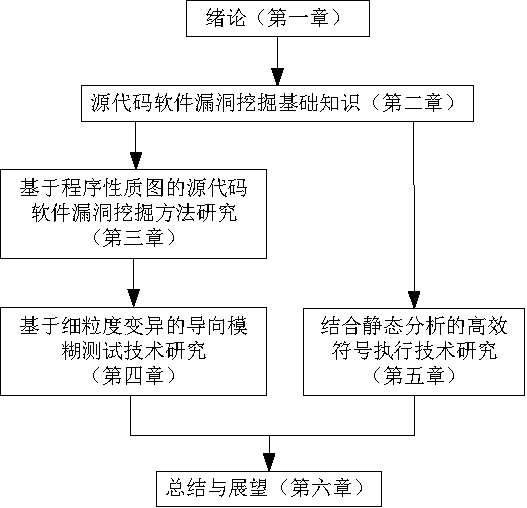
\includegraphics[scale=1.2]{chap01/论文的组织结构}
\end{center}
\caption{论文的组织结构}
\label{论文的组织结构}
\end{figure}
